\state{}{
	The material $\LaSrCuO$ has a layered crystal structure that consists of two-dimensional square lattices of $\CuO$ planes (shown in Fig.~\ref{f1}) separated by layers of $\LaSrO$.  You may assume that $\La$ has valence $3+$, $\Sr$ valence $2+$, and $\Ox$ valence $2-$; the electrons from these cations are donated uniformly to the widely separated $\CuO$ layers, which thus have a two-dimensional electronic structure.  Neutral atomic $\Cu$ has the configuration $[\Ar] 4s^2 3d^9$.  In this compound, four of the $\Cu$ $d$ levels are completely filled, and there is a partially filled band formed from $\dxy$ orbitals.  You may assume the $\Cu$ $4s$ levels are unoccupied, and the $\Ox$ $2p$ levels are fully occupied.  Electronic dispersion perpendicular to the planes may be neglected.
	
	The band structure in the independent particle approximation is well described by a tight-binding model incorporating a single orbital (per unit cell) of $\dxy$ symmetry centered on the $\Cu$ atom, with nonzero Hamiltonian matrix elements $t$ between nearest neighbor orbitals in the $x$ and $y$ directions, and matrix elements $t'$ between second neighbors across the diagonals.
	
	\begin{figure}[b!] \centering
		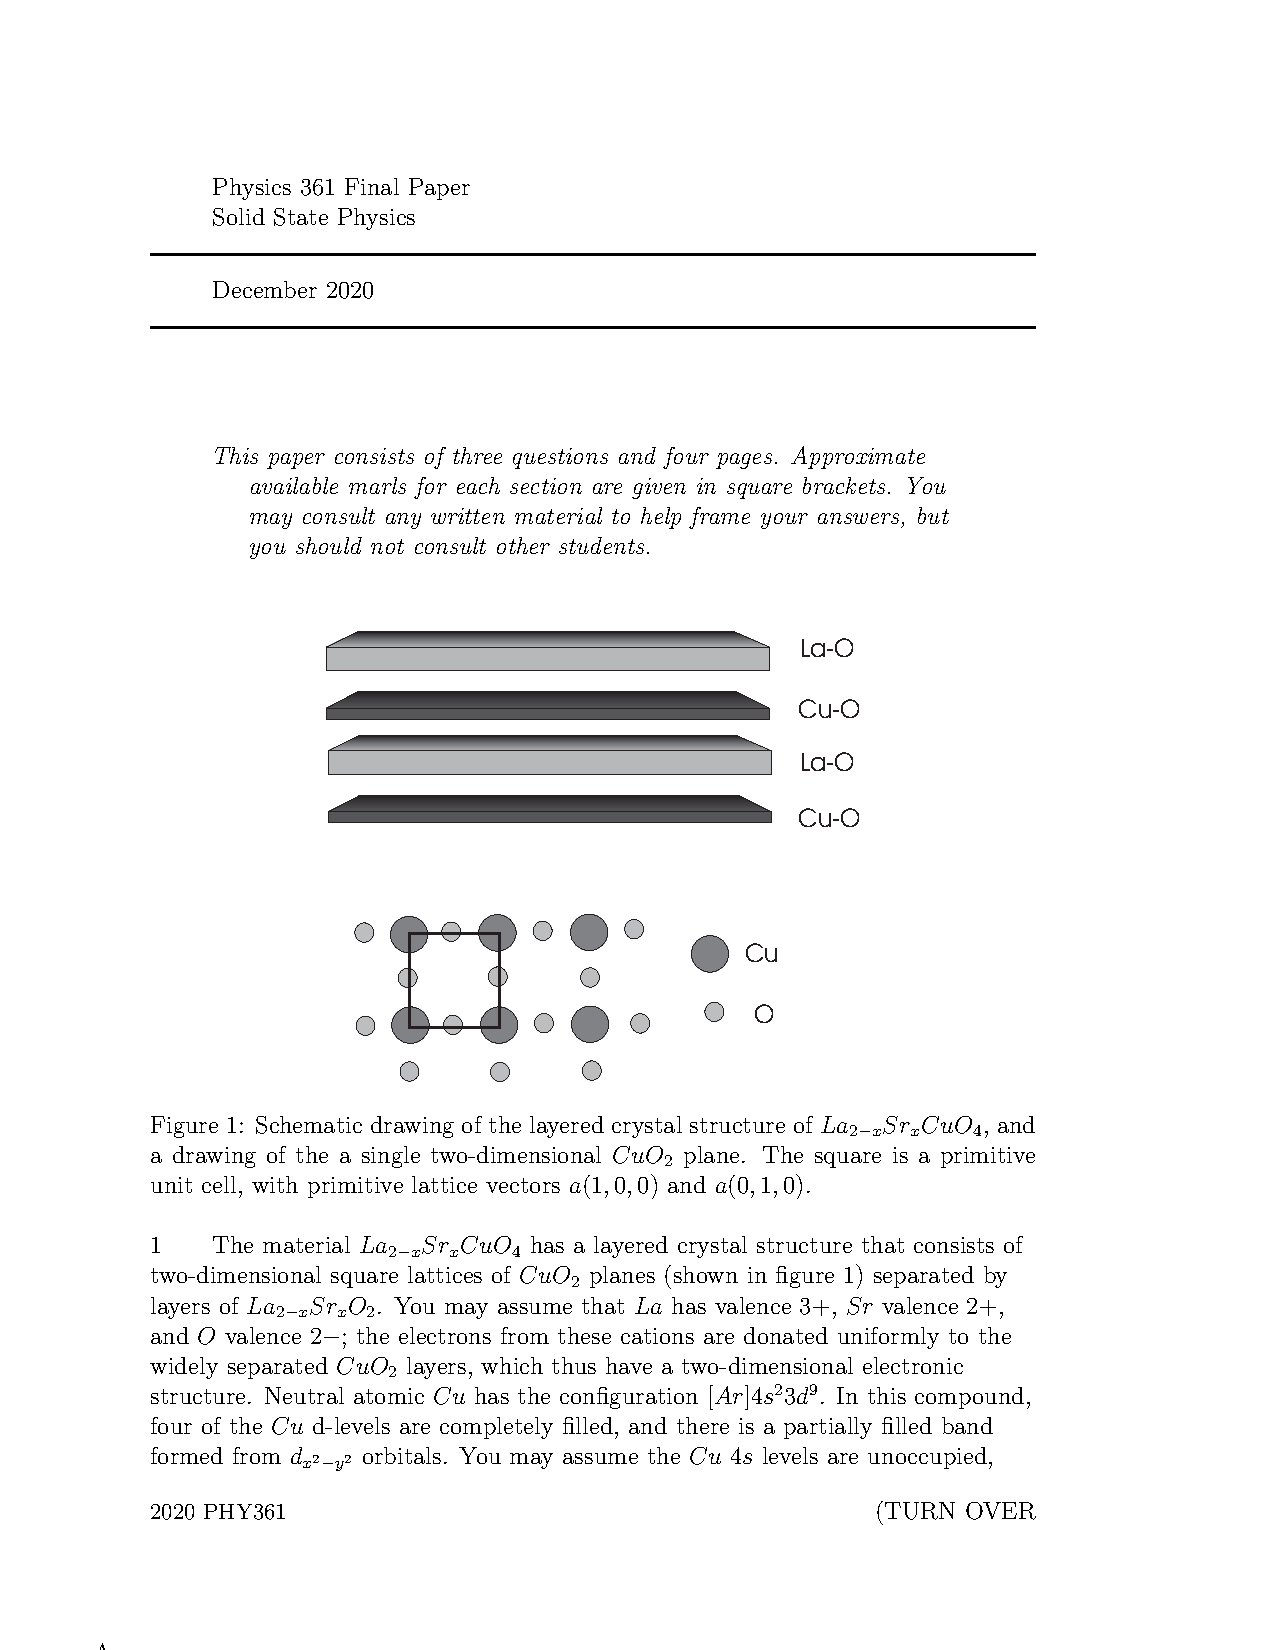
\includegraphics[width=0.5\textwidth,trim=5cm 9.5cm 7cm 10cm,clip]{fig1}
		\caption{Schematic drawing of the layered crystal structure of $\LaSrCuO$, and a drawing of the a single two-dimensional $\CuO$ plane.  The square is a primitive unit cell, with primitive lattice vectors $a(1, 0, 0)$ and $a(0, 1, 0)$.}
		\label{f1}
	\end{figure}
}

\prob{
	Show that in this approximation the energy dispersion of an electron is
	\eq{
		\Ek = 2 t [ \cos(\kx a) + \cos(\ky a) ] + 4 t' \cos(\kx a) \cos(\ky a).
	}
	\vfix
}

\sol{
	The band energy in the tight-binding description is given by (4.57) in the lecture notes,
	\eq{
		\Ek = \epso + t \sumrho e^{-i \vk \vdot \vrho}.
	}
	In the two-dimensional $\CuO$ plane, the four nearest neighbors to the origin are located at
	\eqn{nn}{
		\vrho \in a \{ (1, 0, 0),\ (0, 1, 0),\ (-1, 0, 0),\ (0, -1, 0) \},
	}
	and the four second-nearest neighbors are located at
	\eqn{nnn}{
		\vrho' \in a \{ (1, 1, 0),\ (-1, 1, 0),\ (1, -1, 0),\ (-1, -1, 0) \}.
	}
	So, assuming $\epso = 0$, the band energy is
	\aln{
		\Ek &= t \sumrho e^{-i \vk \vdot \vrho} + t' \sumrhop e^{-i \vk \vdot \vrho'} \notag \\
		&= t \paren{ e^{-i a \kx} + e^{-i a \ky} + e^{i a \kx} + e^{i a \ky} } + t' \paren{ e^{-i a (\kx + \ky)} + e^{i a (\kx - \ky)} + e^{-i a (\kx - \ky)} + e^{i a (\kx + \ky)} } \notag \\
		&= t \paren{ e^{-i a \kx} + e^{i a \kx} + e^{-i a \ky} + e^{i a \ky} } + t' \paren{ e^{-i a \kx} e^{-i a \ky} + e^{i a \kx} e^{-i a \ky} + e^{-i a \kx} e^{i a \ky} + e^{i a \kx} e^{i a \ky} } \notag \\
		&= t \brac{ \paren{ e^{-i a \kx} + e^{i a \kx} } + \paren{ e^{-i a \ky} + e^{i a \ky} } } + t' \paren{ e^{-i a \kx} + e^{i a \kx} } \paren{ e^{-i a \ky} + e^{i a \ky} } \notag \\
		&= t \brac{ 2 \cos(\kx a) + 2 \cos(\ky a) } + t' \brac{ 2 \cos(\kx a) } \brac{ 2 \cos(\ky a) } \notag \\
		&= \ans{ 2 t [ \cos(\kx a) + \cos(\ky a) ] + 4 t' \cos(\kx a) \cos(\ky a) } \label{ans1a}
	}
	as we wanted to show. \qed
}



\prob{ \label{1b}
	What do you expect to be the signs of $t$ and $t'$?  Explain your reasoning.
}

\sol{
	The signs of $t$ and $t'$ are expected to be \ans{negative} because the Coulomb potential $\Del U$ between the two electrons at any two sites is negative~\cite[pp.~78--79]{Coleman}.  We see that $t$ depends on $\Delta U$ by Ashcroft \& Mermin~(10.18), and we see that $t$ has the same sign as $\Del U$ by (4.56) in the lecture notes:
	\eqn{t}{
		t = \int \ddvr \psi^*(\vr - \rho) \Del U \psi(\vr).
	}
	\vfix
}



\prob{ \label{1c}
	For the case that $\abs{t' / t} = 0$, sketch the Fermi surface for $\Sr$ concentrations of $x = 0$, $x \approx 0.2$, and $x \approx 0.5$.
}

\sol{
	As $x$ increases, the partially-filled band of $\Cu$ becomes more empty.  When $x = 0$, $\Cu$ has valence $2+$ and donates its two $4s$ electrons.  This means its $\dxy$ band is half full.  For $x = 0.2$, $\Cu$ has expected valence $2.2+$ and so its $\dxy$ band is expected to be 40\% full.  For $x = 0.5$, $\Cu$ has expected valence $2.5+$ and so its $\dxy$ band is expected to be 25\% full.
	
	Figure~\ref{f1cd}~(left) shows the Fermi surface for $x = 0$~(blue line), $x \approx 0.2$~(gold line), and $x \approx 0.5$~(green line) when $t' = 0$ in the reduced zone scheme~\cite[p.~231]{Kittel}.  The figures were created in Mathematica by plotting Eq.~\refeq{ans1a} and choosing appropriate contours.
}


\begin{figure}[t] \centering
	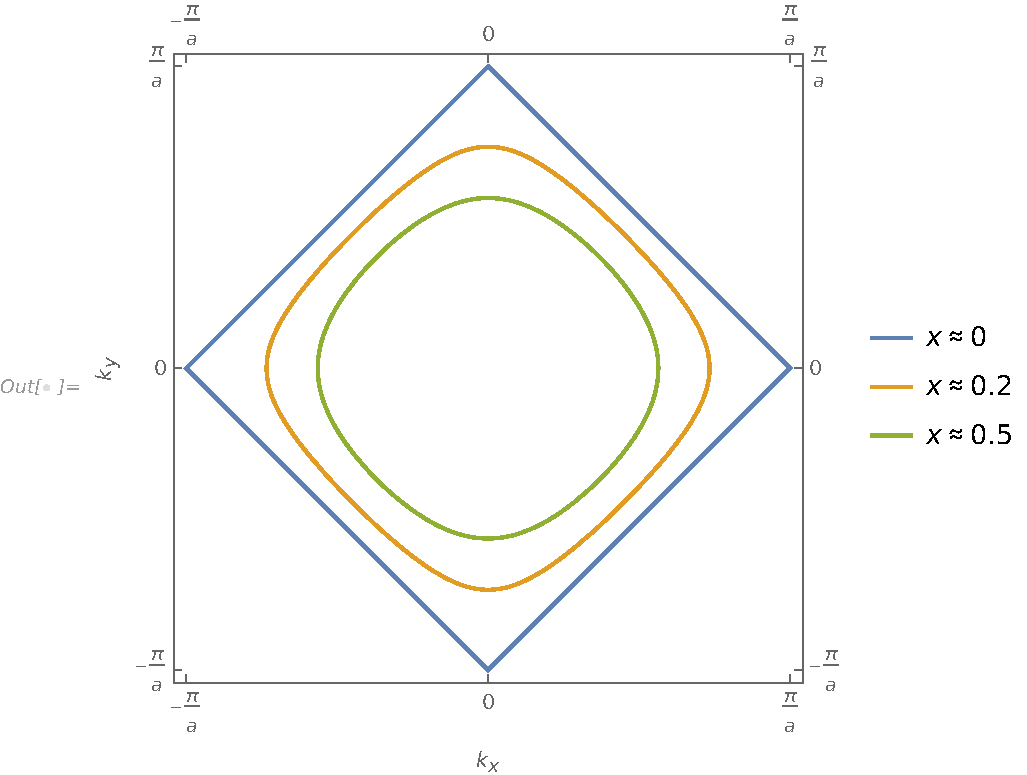
\includegraphics[width=0.49\textwidth,trim=1.5cm 0 0 0,clip]{1c} \hfill
	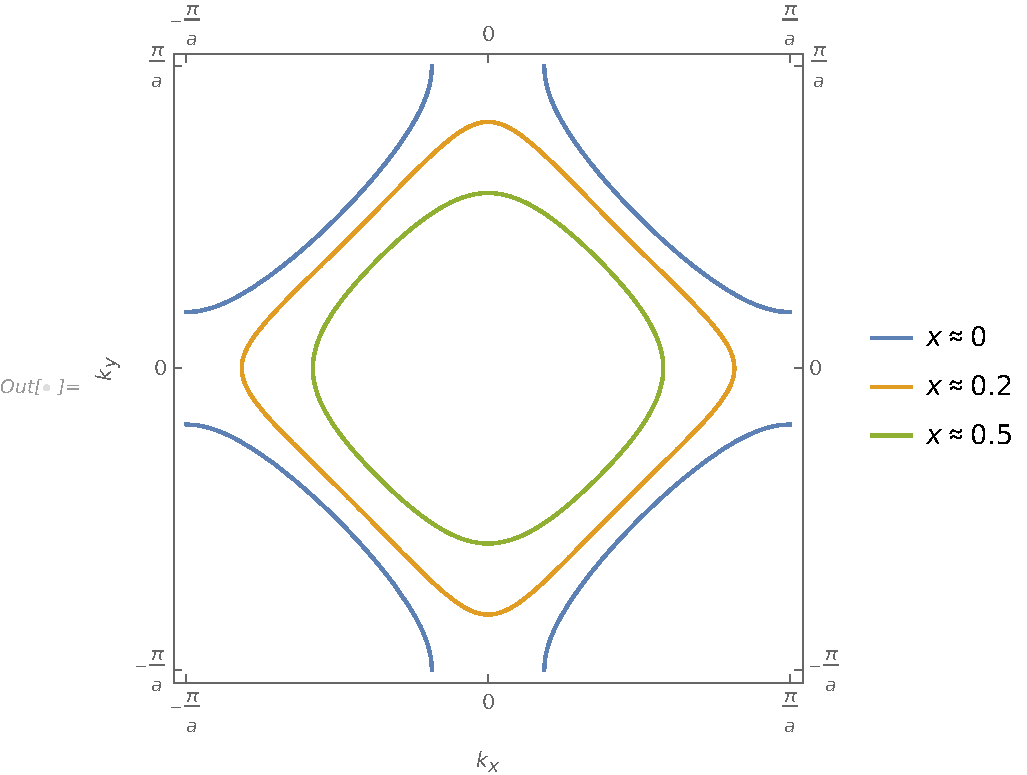
\includegraphics[width=0.49\textwidth,trim=1.5cm 0 0 0,clip]{1d}
	\caption{Fermi surfaces for $t' = 0$~(left) and $\abs{t' / t} = 0.1$~(right) for $x = 0$~(blue line), $x \approx 0.2$~(gold line), and $x \approx 0.5$~(green line).}
	\label{f1cd}
\end{figure}


\prob{ \label{1d}
	How do these contours change qualitatively if $\abs{t' / t} \sim 0.1$?  (Choose the signs of $t$ and $t'$ that you proposed in \ref{1b}.)
}

\sol{
	For $t$ and $t'$ both negative, the contributions from $t'$ will distort the contours by pulling the areas near the ``corners'' of the Fermi surface~(that is, the areas closest to the $\kx$ and $\ky$ axes) toward the corners of the frame.  This happens because, when we consider only $t$ contributions, the Fermi surface is stretched toward the positions of the nearest neighbors (for $t < 0$) given by Eq.~\refeq{nn}.  There is a nearest neighbor at the center of each edge of the frame ($\ki = \pm \pi / a$, $\kj = 0$ for $i \neq j$).  When we also consider $t' < 0$ contributions from the next-nearest neighbors, which are located in the corners of the frame by Eq.~\refeq{nnn}, the Fermi surface is pulled toward those ions as well.  The effect is not too large since $\abs{t'}$ is small compared to $\abs{t}$.
	
	Figure~\ref{f1cd}~(right) shows the Fermi surface in the reduced zone scheme for $x = 0$~(blue line), $x \approx 0.2$~(gold line), and $x \approx 0.5$~(green line) when $t' = 0.1 t$.
}



\prob{
	Assuming the dispersion of \ref{1d}, sketch the electronic density of states in energy, paying particular attention to the behavior near the edges of the band and at a saddle point in the middle of the band.
}

\sol{
	Our sketch of $\gE$ is based on Fig.~4.2 in the course lecture notes, and is shown in Fig.~\ref{f1e}.  The logarithmic singularity in the middle represents the saddle point.  Near the edges, the curve flattens out.

	\begin{figure}[t] \centering
		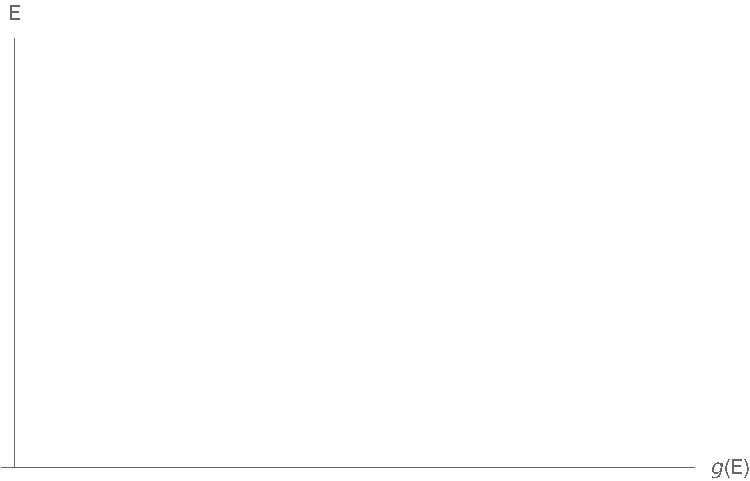
\includegraphics[width=0.5\textwidth]{1e}
		\caption{Density of states $\gE$ for the dispersion shown in Fig.~\ref{f1cd}~(right).}
		\label{f1e}
	\end{figure}
}



\prob{
	What would the independent electron model predict for the temperature dependence of the low-temperature electronic specific heat when the chemical potential is exactly at the saddle point near the middle of the band?
}

\sol{
	By (2.15) in the lecture notes, the electronic specific heat is given by
	\eqn{cv}{
		\cv = \int \ddE E \gE \dv{\fE}{T},
	}
	where $\fE$ is the Fermi distribution, given by (2.12):
	\eqn{fE}{
		\fE = \frac{1}{e^{(E - \mu) / \kB T} + 1}.
	}
	At low temperature, the chemical potential is approximately equal to the Fermi energy, which is reflected in this expression.  The electronic density of states in two dimensions can be found using the result of question~2.2(b) of the homework:
	\eqn{gE}{
		\gE = 2 \frac{2 \pi k}{(2\pi)^2} \dv{k}{E}.
	}
	The saddle points are located at the positions of the nearest neighbors, given by Eq.~\refeq{nn}.  Since the lattice is periodic, there is really only one saddle point per unit cell, so we can choose $\vk = (0, \pi / a, 0)$ without loss of generality~[lecture notes, p.~18].  Now we expand Eq.~\refeq{ans1a} about this point in order to find an approximation for $\gE$.  Let $\vk \to \vk + \del\vk$:
	\eqn{thing1f}{
		\Ek \approx 2 t [ \cos(\del k a) + \cos(\pi + \del k a) ] + 4 t' \cos(\del k a) \cos(\pi + \del k a).
	}
	The Taylor series expansion of $\cos(x)$ about $x = 0$ is~\cite{Maclaurin}
	\eq{
		\cos(x) = 1 - \frac{x^2}{2} + \cdots.
	}
	Now we substitute this result into Eq.~\refeq{thing1f}.  In order to find a $\dv*{E}{k}$ that is independent of $k$, we must neglect terms of $\order{\del k^2}$:
	\al{
		\Ek &\approx 2 t \paren{ 1 - \frac{(\del k a)^2}{2} + 1 - \frac{(\pi + \del k a)^2}{2} } + 4 t' \paren{ 1 - \frac{(\del k a)^2}{2} } \paren{ 1 - \frac{(\pi + \del k a)^2}{2} } \\
		&\approx 2 t \paren{ 2 - \frac{\del k^2 a^2}{2} - \frac{\pi^2 + 2 \pi \del k a + \del k^2 a^2}{2} } + 4 t' \paren{ 1 - \frac{\del k^2 a^2}{2} } \paren{ 1 - \frac{\pi^2 + 2 \pi \del k a + \del k^2 a^2}{2} } \\
		&\approx 2 t \paren{ 2 - \frac{\pi^2 + 2 \pi \del k a}{2} } + 4 t' \paren{ 1 - \frac{\pi^2 + 2 \pi \del k a}{2} } \\
		&\approx 4 (t + t') - (\pi^2 + 2\pi \del k a) (t + 2 t').
	}
	Then
	\eq{
		\dv{E}{k} \approx -2 \pi^2 a (t + t'),
	}
	so from Eq.~\refeq{gE},
	\eq{
		\gE = -\frac{k}{2 \pi^3 a (t + t')}.
	}
	Since the two-dimensional Fermi sphere has area $\pi \kF^2$ as seen in question~2.2(b),
	\eq{
		\gE = \frac{E}{4 \pi^4 a^2 (t + t')^2}.
	}
	Feeding this and Eq.~\refeq{fE} into Eq.~\refeq{cv}, we find
	\eqn{thing1f2}{
		\cv = \frac{1}{4 \pi^4 a^2 (t + t')^2} \dv{T} \intoi \ddE \frac{E^2}{e^{(E - \mu) / \kB T} + 1}.
	}
	An integral of the form
	\eq{
		I = \intoi \ddeps \frac{\feps}{e^{(\eps - \mu) / T} + 1},
	}
	where $\feps$ is an arbitrary function, can be expanded for small $T$ as~\cite[p.~155]{Landau}
	\eq{
		I = \intomu \feps \ddeps + \frac{\pi^2}{6} T^2 f'(\mu) + \frac{7 \pi^4}{360} T^4 f'''(\mu) + \cdots.
	}
	Using this in Eq.~\refeq{thing1f2} where $\feps = \eps^2$ with $T \to \kB T$, we find that
	\eq{
		\cv \approx \frac{1}{4 \pi^4 a^2 (t + t')^2} \dv{T}(\intomu E^2 \ddE + \frac{\pi^2}{6} T^2 (2 \mu) )
		= \frac{1}{4 \pi^4 a^2 (t + t')^2} \paren{ \frac{2 \pi^2}{3} T \mu }
		= \ans{ \frac{\mu T}{6 \pi^2 a^2 (t + t')^2}. }
	}
	So the temperature dependence of the specific heat is linear in this regime.
}



\prob{
	$\LaCuO$ is an antiferromagnetic insulator.  Suggest, and discuss, reason(s) why the ground state differs from that predicted by the band structure in the independent particle approximation.  Your answer should include a qualitative explanation of both the magnetic and the insulating behavior.
}

\sol{
	In the independent particle approximation, we expect $\LaCuO$ to be a metal because it has a Fermi surface as we determined in \ref{1c} and \ref{1d}~[lecture notes, p.~39].  However, our illustration of the Fermi surface rests upon the assumption in the tight-binding model that it is a reasonable approximation to treat the atomic state as a non-degenerate $s$ statel~[lecture notes, pp.~46--48].  The actual orbital in question here is a $d$ orbital which may be highly degenerate.  Moreover, our determination of the signs of $t$ and $t'$ is based on Eq.~\refeq{t}, which is based on the $s$ state.  For the actual $d$ state, $t$, $t'$, and $t' / t$ may very well have different signs, so the Fermi surface may look different from what is shown in Fig.~\ref{1d}.
	
	In order for $\LaCuO$ to have insulating behavior instead of conducting behavior, it would need a band gap~[lecture notes, p.~39].  It is possible that the electron-electron interactions in $\LaCuO$ cause its electrons to distribute themselves in such a way such that the $3d$ band is effectively split into two (or more) energy levels with a gap between them.  That is, due to Coulomb repulsion, it may cost so much energy to add the final electron that it can be considered to occupy a higher energy state.  This creates an effective band gap and makes the material a Mott insulator~[lecture notes, p.~111] \cite{Mott}.
	
	As we would expect $\LaCuO$ to be a metal, we would expect it to exhibit Pauli paramagnetism~[lecture notes, p.~113].  If instead it is antiferromagnetic, one way this antiferromagnetism may come about is via superexchange.  This is likely for $\LaCuO$ because the two magnetic $\Cu$ ions are separated by $\Ox^{2-}$ ions, which are nonmagnetic ions with closed shells~[lecture notes, p.~110--111].  This behavior would not come about in the independent particle approximation because it does not take into account ion-ion interactions like superexchange.
}